% $Id: board2.tex 9375 2021-08-31 13:01:06Z mskala $

%
% MSK 007 Board 2 build instructions
% Copyright (C) 2017, 2021  Matthew Skala
%
% This program is free software: you can redistribute it and/or modify
% it under the terms of the GNU General Public License as published by
% the Free Software Foundation, version 3.
%
% This program is distributed in the hope that it will be useful,
% but WITHOUT ANY WARRANTY; without even the implied warranty of
% MERCHANTABILITY or FITNESS FOR A PARTICULAR PURPOSE.  See the
% GNU General Public License for more details.
%
% You should have received a copy of the GNU General Public License
% along with this program.  If not, see <http://www.gnu.org/licenses/>.
%
% Matthew Skala
% https://northcoastsynthesis.com/
% mskala@northcoastsynthesis.com
%

\chapter{Building Board 2}

There are a few header connectors which serve to link the boards together. 
My recommendation is to solder in the three links to Board~3 while working
on Board~2, and accordingly, the partial Bill Of Materials in
Table~\ref{tab:b2bom} includes these connectors.  The link to Board~1 will
be left for later.

Note that although I'm describing a separate step for each component value,
and that's how I built mine so as to have plenty of photo opportunities, if
you are reasonably confident about your skills you may find it easier to
populate all or most of the board (i.e.\ put the components in place) and
then solder them in a single step.  Except where noted, the order in which
you add components does not matter much.

\section{Preliminaries}

Count out the right number of everything according to the bill of materials. 
There is an abbreviated BOM for Board~2 alone in Table~\ref{tab:b2bom},
including some hardware that will be useful for this part of the build but
overlaps with the requirements for other boards.  In addition to these
things you will need your assembled Board~3 from the previous chapter.

\noindent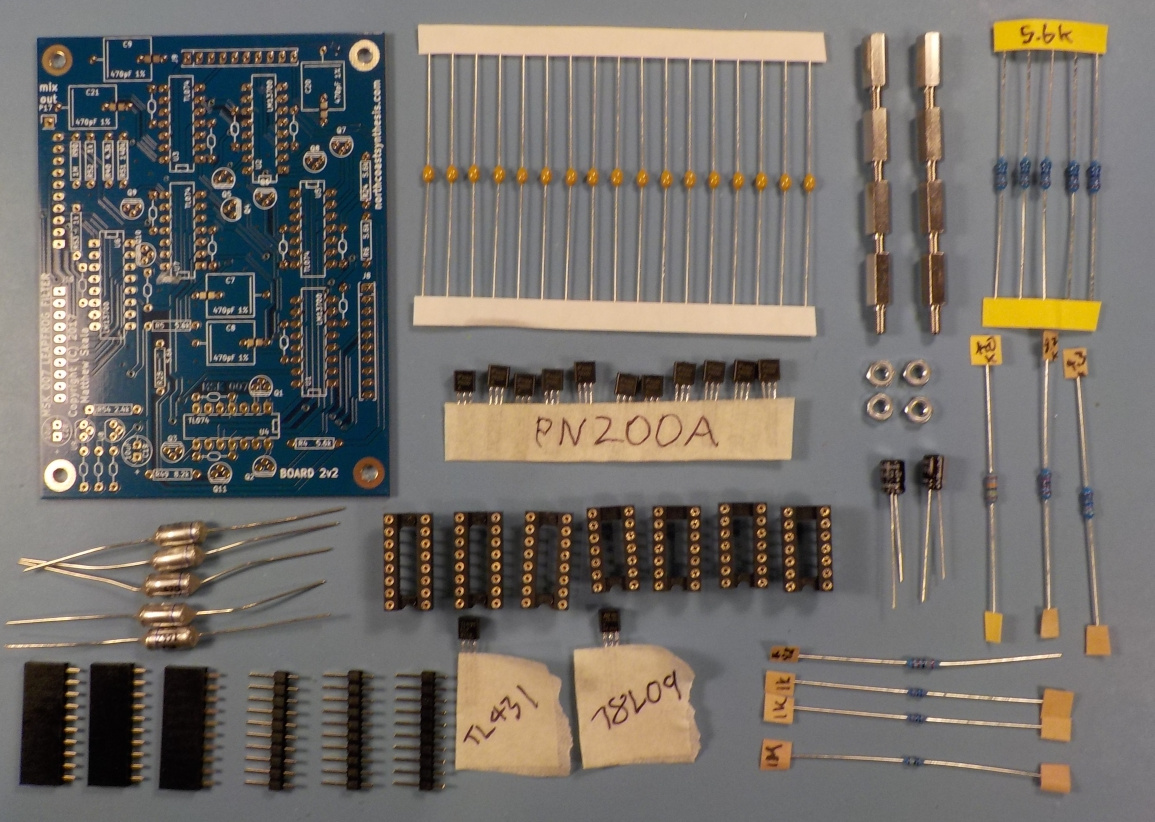
\includegraphics[width=\linewidth]{board2-parts.jpg}

\begin{table*}
{\centering
\fbox{This table is not a substitute for the text instructions.}
\vspace{\baselineskip}

\begin{tabular}{rp{1in}cp{3in}}
  \textbf{Qty} & \textbf{Ref} & \textbf{Value/Part No.} & \\ \hline
\input{bomdata-2.tex}
\end{tabular}\par}
\caption{Bill of Materials for Board~2.}\label{tab:b2bom}
\end{table*}

\newpage

\section{Fixed resistors}

Resistors are never polarized.  I like to install mine in a consistent
direction for cosmetic reasons, but this is electrically unnecessary.  In
this module, metal film 1\%\ resistors are recommended for all fixed-value
resistors.  These will usually have blue bodies and four colour bands
designating the value, plus a fifth band for the tolerance, brown in the
case of 1\%.  These are the resistors normally shipped in the
North Coast kits, but we may occasionally ship better-tolerance resistors (such
as 0.5\%) if we are able to source them at a good price. 
Accordingly, I mention only the four value band colours for this type of
resistor; if you are using resistors with other codes, you are responsible
for knowing them.  Note that colour codes on metal film 1\% resistors are
often ambiguous (reading from one end or the other end may give two
different values, both plausible) and some of the colours are hard to
distinguish anyway.  If in doubt, always measure with an ohmmeter before
soldering the resistor in place.

Install the two 1k$\Omega$ (brown-black-black-brown) resistors R52 and R53. 
These are input resistors for the OTA in the VCA section.  After installing
them, and the ten 1k$\Omega$ resistors on Board~3, one more 1k$\Omega$
resistor should remain for use on Board~1.

\nopagebreak
\noindent\includegraphics[width=\linewidth]{{res-1.0k2}.jpg}

\pagebreak

Install the 2.4k$\Omega$ (red-yellow-black-brown) resistor R54.  This
resistor provides a minimum load for the TL431 voltage regulator.

\nopagebreak
\noindent\includegraphics[width=\linewidth]{{res-2.4k2}.jpg}

Install the 4.3k$\Omega$ (yellow-orange-black-brown) resistor R40.  This
is the feedback resistor that sets overall gain for the output mixer.

\nopagebreak
\noindent\includegraphics[width=\linewidth]{{res-4.3k2}.jpg}

\pagebreak

Install the five 5.6k$\Omega$ (green-blue-black-brown) resistors R4 to R6,
R24, and R25.  These are references for the control current generators, one
per integrator.  One more 5.6k$\Omega$ resistor should remain for use on
Board~1.

\nopagebreak
\noindent\includegraphics[width=\linewidth]{{res-5.6k2}.jpg}

Install the 8.2k$\Omega$ (grey-red-black-brown) resistor R49.
This resistor sets the linearizing diode current for the VCA section.

\nopagebreak
\noindent\includegraphics[width=\linewidth]{{res-8.2k2}.jpg}

\pagebreak

Install the 140k$\Omega$ (brown-yellow-black-orange) resistor R51.  This is
part of the input voltage divider for the LM13700 half in the VCA section.

\nopagebreak \noindent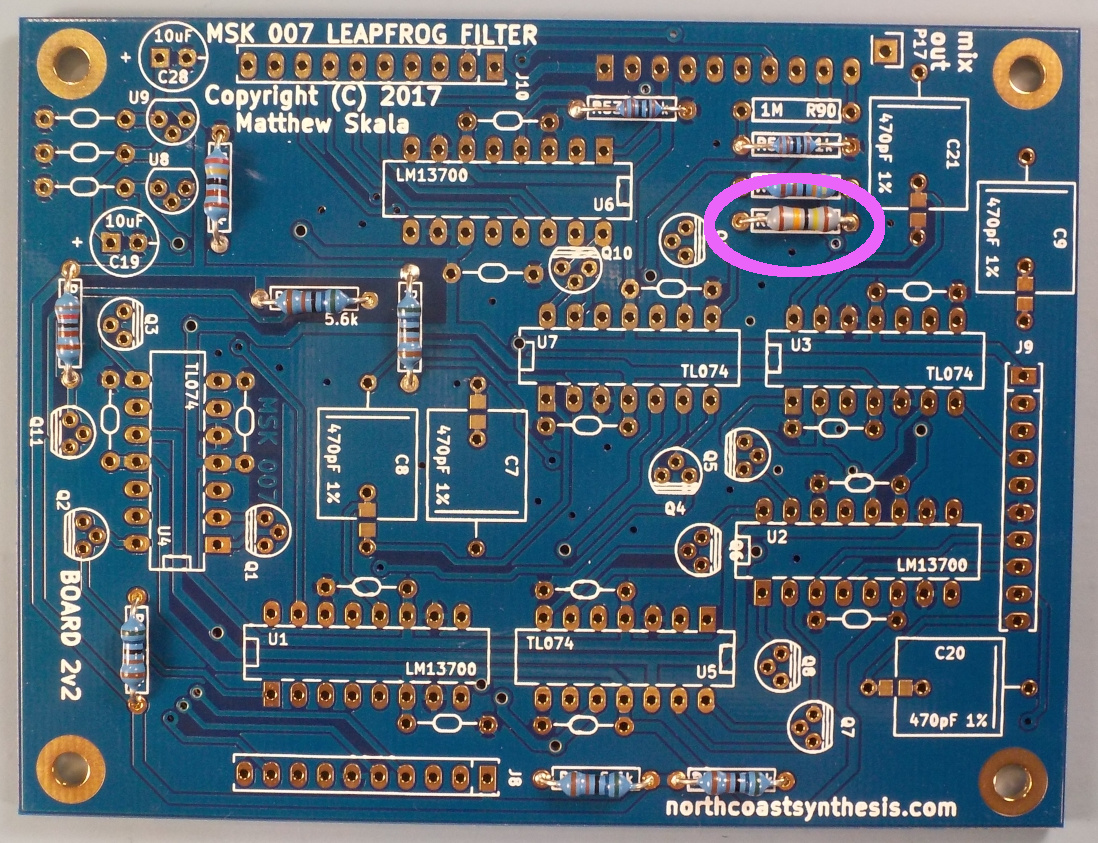
\includegraphics[width=\linewidth]{res-140k2.jpg}

Install the 1M$\Omega$ (brown-black-black-yellow) resistor R90.  This
controls the range for the VCA offset trimmer.

\nopagebreak \noindent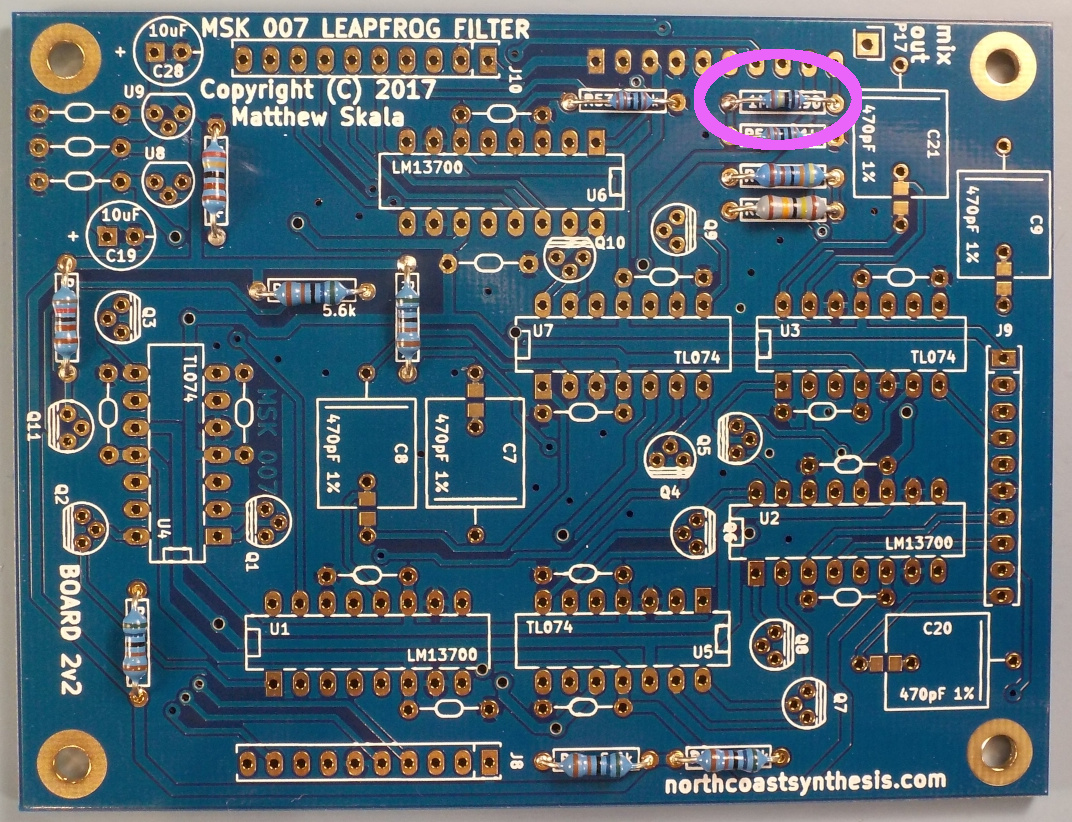
\includegraphics[width=\linewidth]{res-1m2.jpg}

\section{DIP sockets}

Install the four 14-pin DIP sockets for the TL074 quad op amp chips U3 to U5
and U7.  These amplifiers are used for multiple purposes throughout the
filter core.  One more 14-pin DIP socket should remain for use on Board~1.

The sockets\label{pag:dip-sockets} themselves do not care which direction
you install them, but it is critically important that the chips installed in
the sockets should be installed in the right direction.  To help with that,
the sockets will probably be marked with notches at one end (indicating the
end where Pin~1 and Pin~14 are located) and you should install the sockets
so that the notched ends match the notches shown on the PCB silkscreen.  The
solder pad for Pin~1 is also distinguished by being rectangular instead of
rounded.

Installing DIP sockets without having them tilted at a funny angle can be
tricky.  I recommend inserting the socket in the board, taping it in place
on the component side with vinyl electrical tape, then soldering one pin on
one corner and checking that the socket is snug against the board before
soldering the other pins.  That way, if you accidentally solder the first
pin with the socket tilted, it will be easier to correct (only one pin to
desolder instead of all of them).

If you somehow manage to solder an entire socket in backwards, don't try to
desolder it to turn it around.  Just leave it as it is and remember
when you insert the chip to insert it so the chip matches the
markings on the \emph{board}, not the socket.

\noindent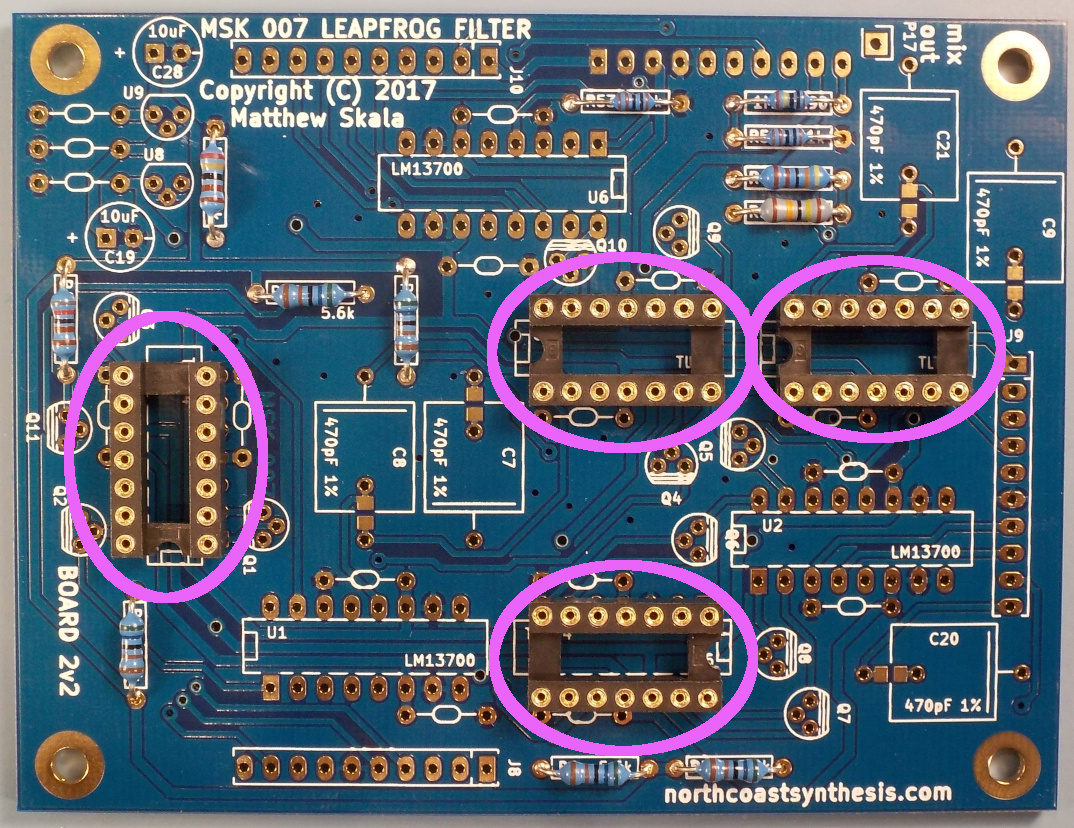
\includegraphics[width=\linewidth]{dip14-2.jpg}

Install the three 16-pin DIP sockets for the LM13700 dual operational
transconductance amplifier chips U1, U2, and U6.  These current-controlled
amplifiers provide variable amplification for the filter core and VCA
section.

\noindent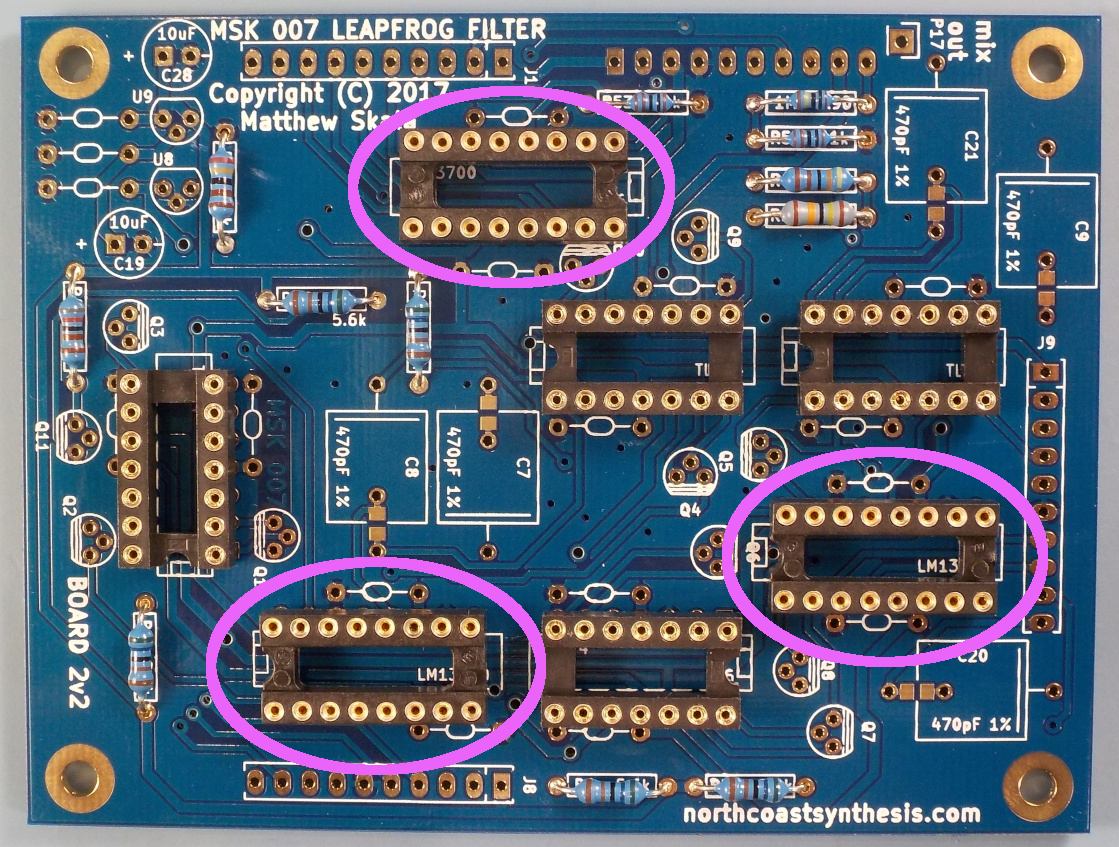
\includegraphics[width=\linewidth]{dip16-2.jpg}

\section{Decoupling capacitors}

The 17 axial ceramic 0.1$\mu$F decoupling capacitors are shown on the board
by a special symbol without their reference designators.

\noindent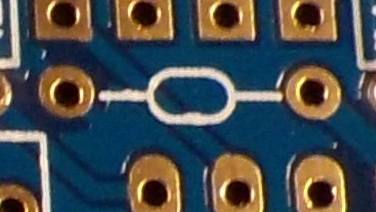
\includegraphics[width=\linewidth]{decoup-symbol.jpg}%
\label{pag:decoup-symbol}

Install these capacitors where the symbol appears.  They are not polarized
and may be installed in either orientation.  Most of these capacitors act as
filters for the power supplies to the amplifier chips, reducing any coupling
of high-frequency noise between them and the rest of the synthesizer.  Three
perform a similar function for the voltage regulators.  A
full MSK~007 kit should contain 19 of these capacitors, leaving two for use
on Board~1.

\noindent\includegraphics[width=\linewidth]{{cap-0.1u2}.jpg}

\section{TO-92 semiconductors}\label{sec:to92-2}

The MSK~007 contains four different types of components packaged in TO-92
packages, of which three types are used on Board~2.\label{pag:to-92}
Each such component
looks like a little black pill of epoxy plastic with one flat side and three
metal legs; they can be distinguished by etched or printed numbers on the
flat side, and it is important to sort them carefully and install only the
proper component type in each footprint.

\pagebreak

There is not enough space on the boards to print a part number for every
TO-92 component, but there are two different silkscreen symbols used to help
with recognition.  The PNP transistors, which are the most numerous type
in this project, are shown on the board with extra silkscreen lines along
the flat edge, as in the left photo.  All other TO-92 components (78L09,
TL431, and 2N5088 which is not used on Board~2) are shown by a plain outline
without extra lines, as in the right photo.

\noindent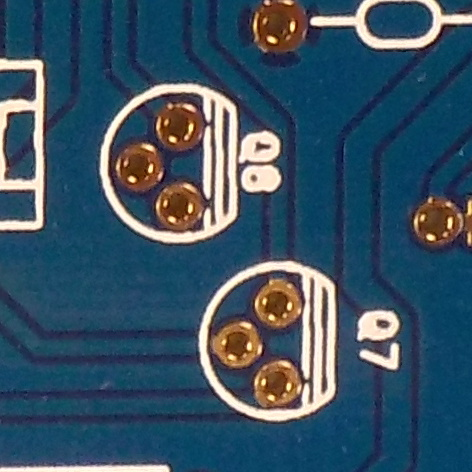
\includegraphics[width={1.50in}]{to92-bar.jpg}\quad
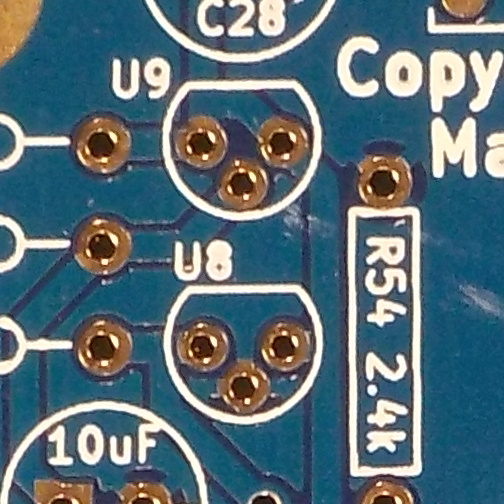
\includegraphics[width={1.50in}]{to92-nobar.jpg}

All TO-92 components in this project are polarized and must be installed in
the correct orientation to work; that orientation is shown by the silkscreen
symbols.  Install each component so that its fully flat side points in the same
direction as the flat side shown on the silkscreen.  The three legs of the
component must be carefully bent into the same triangular pattern (left and
right forward, middle backward) as the holes on the board, and then the
component pressed into place.  There should be a gap of about three
millimetres between the board and the component body; do not attempt to seat
the component flush on the board because of the risk of breaking off the
legs where they enter the body.

The solder pads for TO-92 components are smaller and closer together than
for any other through-hole components in the project, and the components
themselves tend to be relatively heat-sensitive.  Solder them carefully,
avoiding creating any solder bridges between adjacent pads.  Do not use
excessive time and heat trying to get the solder to flow through the board
and fillet on both sides, especially not on pads connected to the ground
plane; two-sided fillets may happen naturally, but it is enough for solder
to completely cover the pad on one side.

\pagebreak

Install the eleven PNP transistors, type SS8550D or PN200A with references
Q1 through Q11.  These are all used as current sources for biasing the
LM13700 chips.  There should be one more PNP transistor remaining for
installation on Board~1.

\nopagebreak
\noindent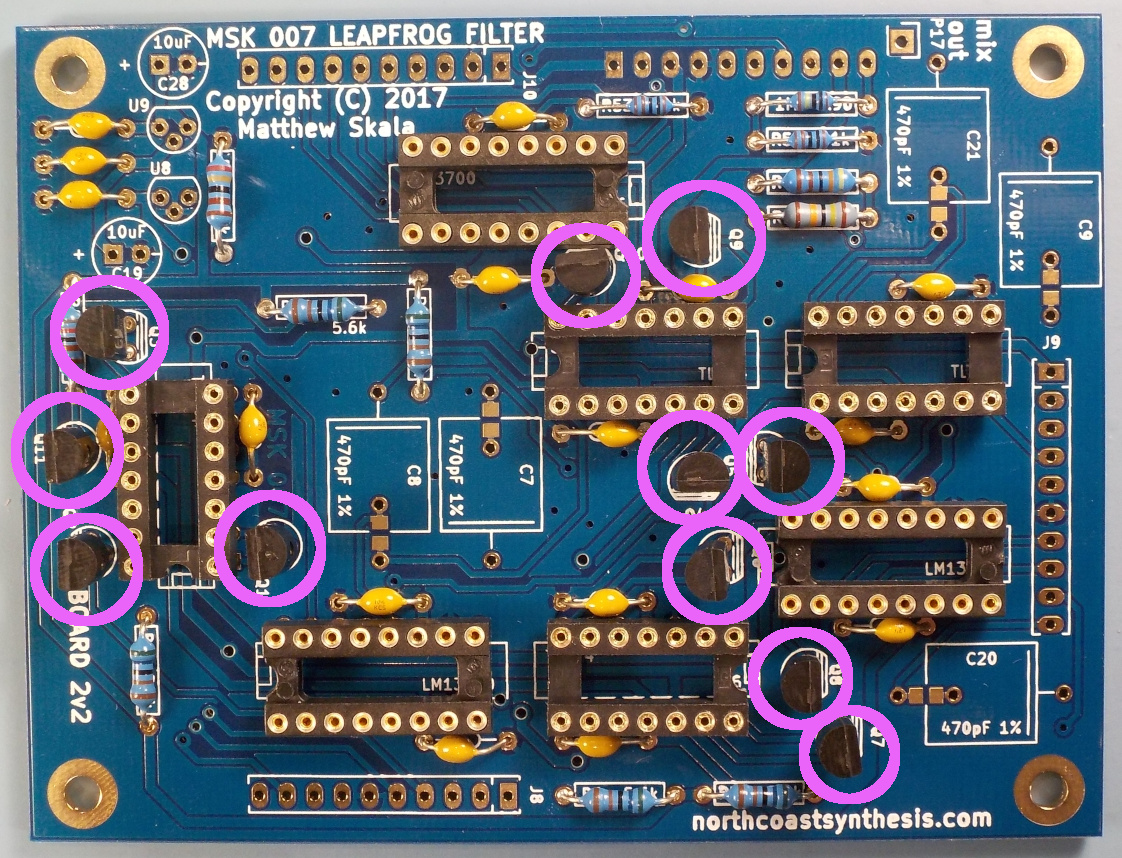
\includegraphics[width=\linewidth]{pn200a-2.jpg}

Install the 78L09 voltage regulator IC, U8.  Be sure not to confuse it with
the nearby symbol for the other voltage IC.  This regulator controls an
internal voltage bus from which all the control currents are drawn,
helping to isolate the filter core from the system power supply.

\nopagebreak
\noindent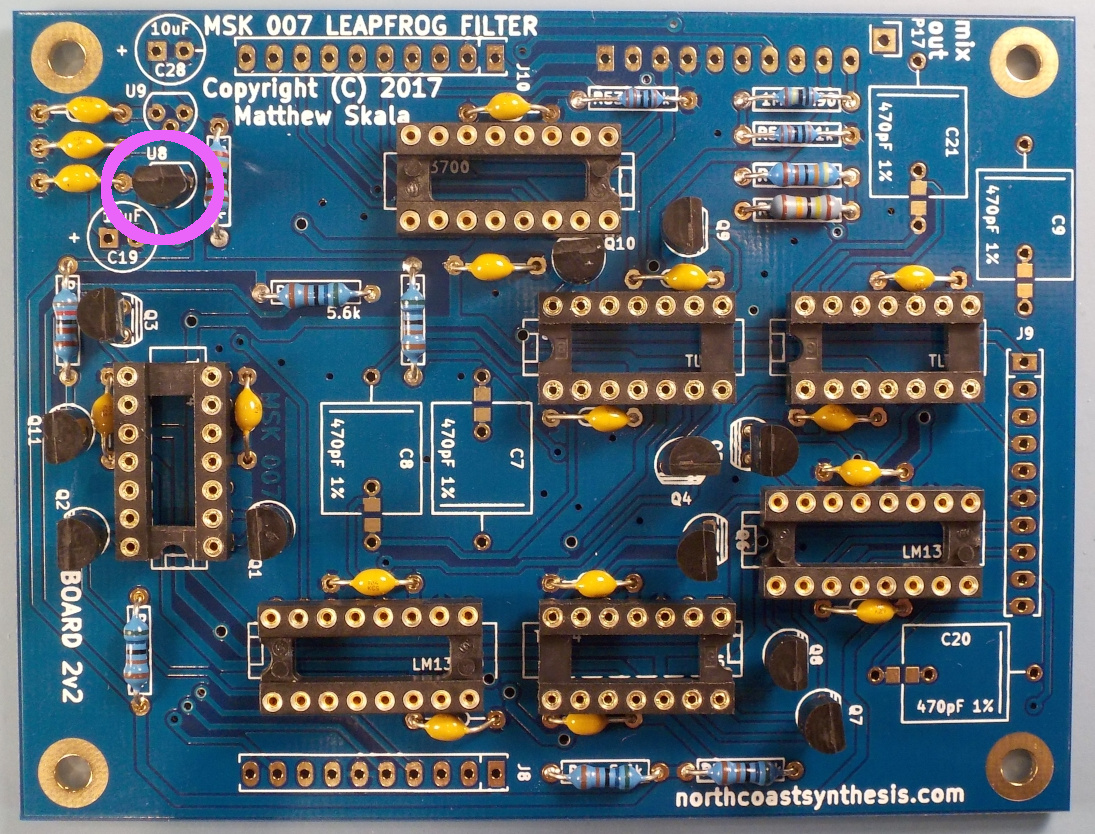
\includegraphics[width=\linewidth]{78l09.jpg}

\pagebreak

Install the TL431 voltage reference IC, U9.  This IC controls another
internal voltage bus, nominally $+$6.5V but really defined by its difference
from the $+$9V bus.  The difference between the two busses is used as a
reference for the voltage-to-current converters that mirror the module
tuning to control the five integrators of the filter core.

\nopagebreak
\noindent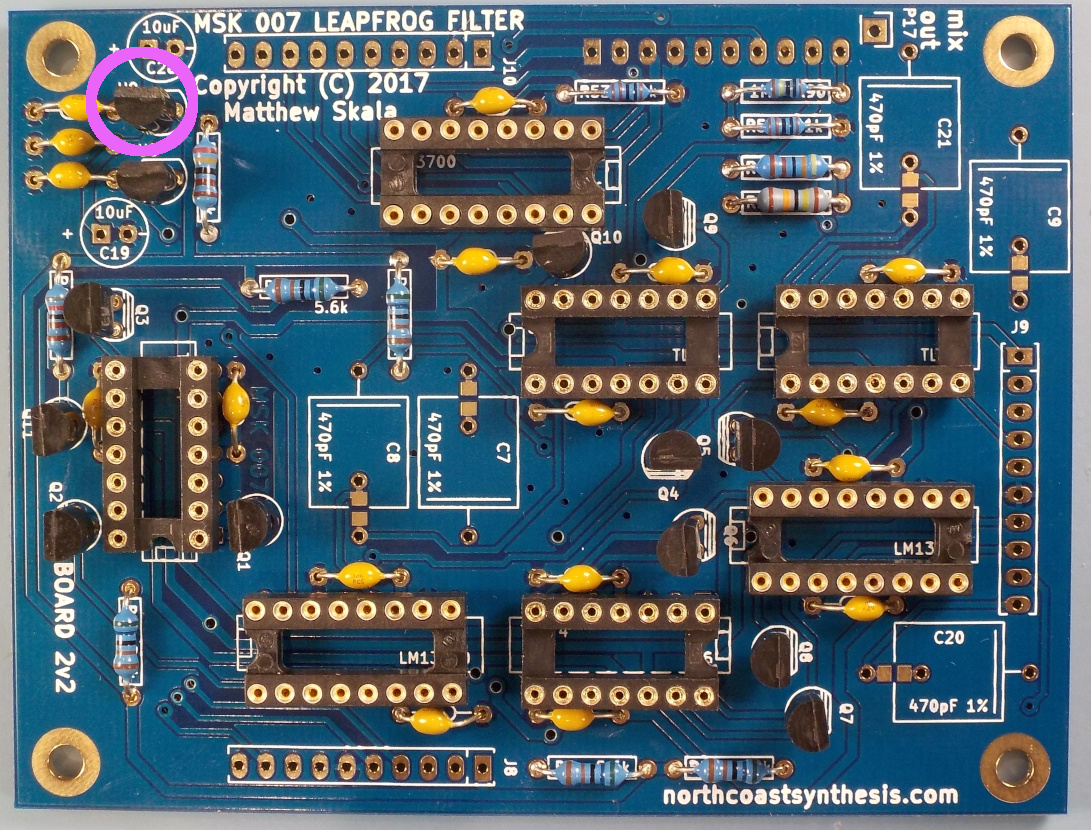
\includegraphics[width=\linewidth]{tl431.jpg}

\section{Integrator capacitors}

Install the five integrator capacitors C7, C8, C9, C20, and C21.  These
store voltages that directly represent the ``state variables'' by which the
filter calculates its response.  Each footprint has extra holes and pads to
allow options for mounting a through-hole capacitor with 0.2$''$ or 0.6$''$
lead spacing, or a surface-mount chip of reasonable size.  The polystyrene
capacitors recommended as defaults and included in North Coast kits should
be mounted in the 0.6$''$ holes.  See page~\pageref{pag:integrator-sub} for
notes on capacitor substitution options.

\nopagebreak
\noindent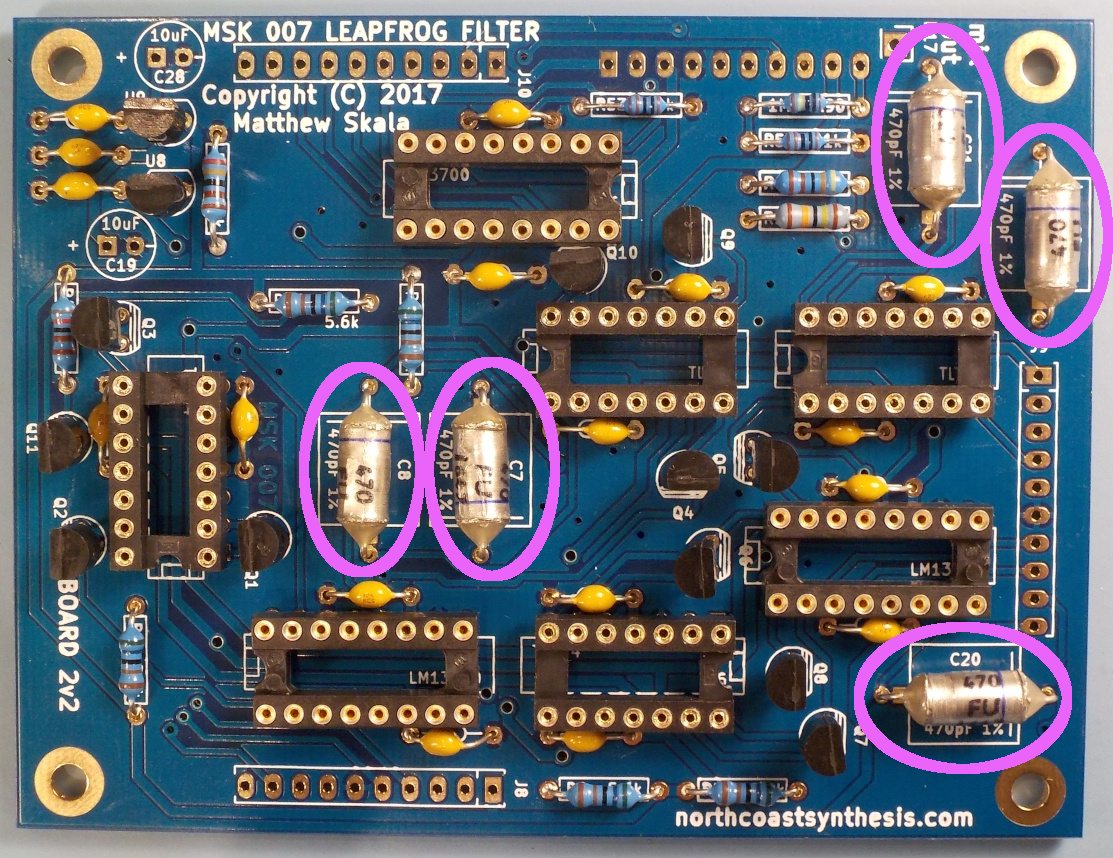
\includegraphics[width=\linewidth]{cap-470p.jpg}

\pagebreak

The polystyrene capacitors are expensive and delicate.  Do not overheat them
while soldering; do not use extra time and heat trying to get the solder to
go through the board and fillet on both sides.  You may wish to use a
clip-on heat sink on the component side of the board while soldering, to
reduce the exposure of the capacitor body to the soldering heat.  Devices
made specifically for this purpose are available from the same suppliers as
other soldering accessories, but it also works to simply clip on the kind of
alligator clip used for electronic testing.

Although these capacitors are not polarized as such, and polarized
capacitors should not be substituted here, axial film capacitors do usually
have a marking at one end (often a dark stripe) which indicates the end
connected to the outermost foil wrap.  It's better for that end to be
connected to ground potential.  If your capacitors have such a marking,
install them so that the marking matches the similar marking on the PCB
footprint, to reduce the voltage between the outside of the capacitor and
the nearby ground plane.  In this particular circuit, this measure is
unlikely to make any real difference, but given that you have a choice about
which way to install the components, it makes sense to do it right.

\newpage

\section{Electrolytic capacitors}

Install the two 10$\mu$F electrolytic capacitors C19 and C28.  These filter
the 9V and 6.5V reference voltages and ensure stability of the regulators
that control those busses.  They are polarized components, and may explode
if connected backwards.  As such, there are multiple clues to help you
install them in the right direction.  The negative leg of each capacitor
will be marked in some way, usually with a printed stripe and minus signs on
the plastic wrapping of the capacitor body.  The negative leg of the
capacitor will usually also be shorter, though that is less reliable than
the body markings.  On the PCB, the positive and negative pads are marked
with positive and negative signs in the silkscreen, and the solder pads
themselves are round for negative and square for positive.

\noindent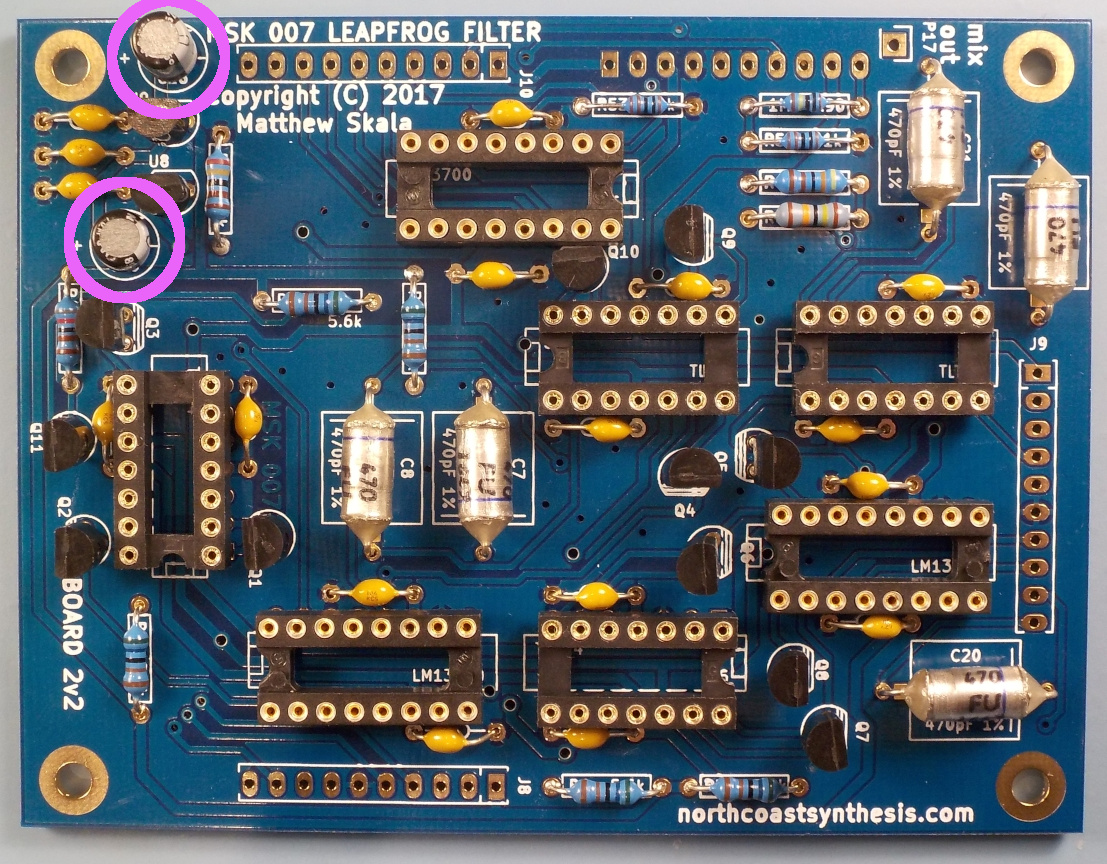
\includegraphics[width=\linewidth]{cap-10u2.jpg}

\pagebreak

\section{Connection to Board~3}

Mate the 10$\times$1 header connectors J8, J9, J10, P40, P42, and P44 into
pairs and assemble Boards~2 and~3 with the three pairs of connectors
sandwiched between them as shown.  The female connectors should be on
Board~2 and the male ones on Board~3.

\noindent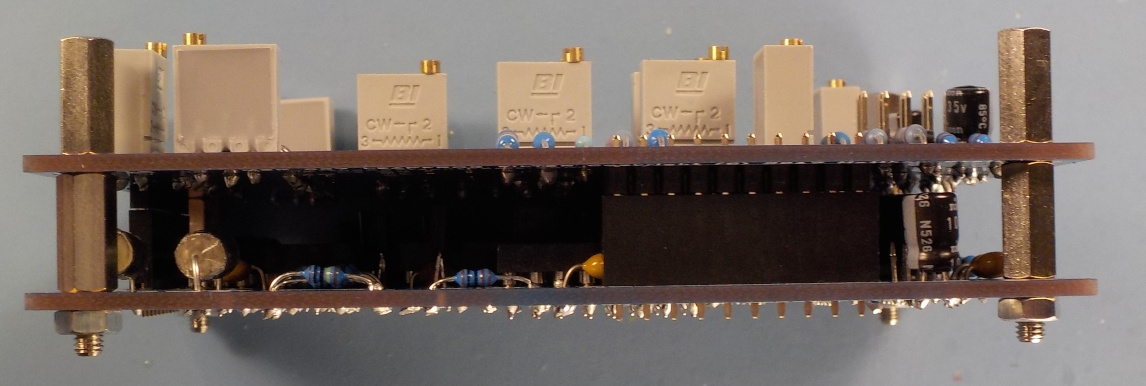
\includegraphics[width=\linewidth]{board23-stack.jpg}

Use four 11mm standoffs to separate the boards.  The hex nuts and additional
11mm standoffs are listed on the BOM for temporary use in making this
assembly; I suggest using standoffs for this because they are easier to
assemble by hand for a temporary assembly than machine screws, and 11mm in
particular to reduce the possibility for confusing the different sizes in
the kit.  For reference, here are the positions of the connectors on Board~2.

\noindent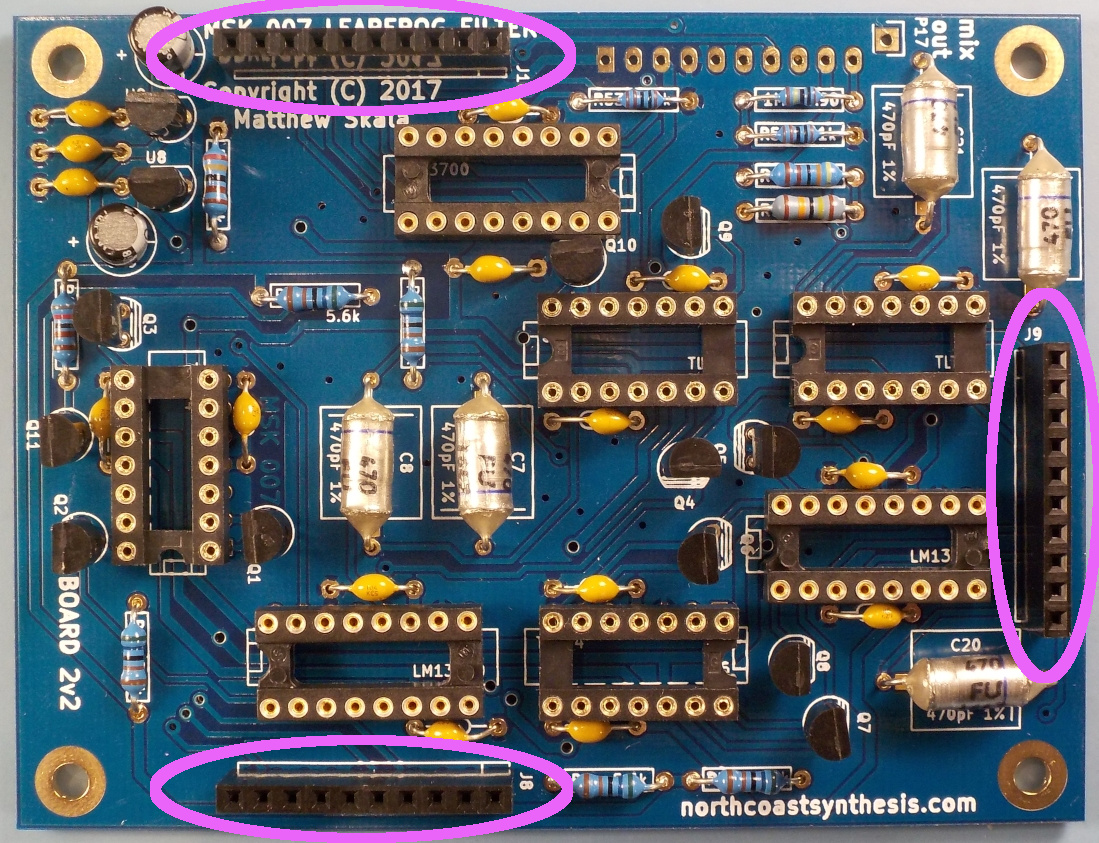
\includegraphics[width=\linewidth]{10x1-2.jpg}

Solder the connectors and then unscrew the temporary assembly and carefully
separate the boards.  You have finished Board~2, except for the connection
to Board~1 which will be made later.  In between completed boards is a good
time to take a break.
